\begin{figure}[h!t]
      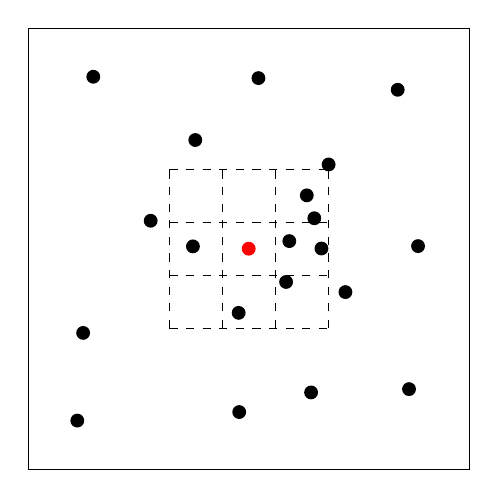
\begin{tikzpicture}[scale=1.12]%[scale=1.055]
        \pgfmathsetseed{5}
        \tikzstyle{every node}= [circle,fill=black, minimum size= 5pt,inner sep=0pt];
        \foreach \x in {1,2,3,4}{
          \foreach \y in {1,2,3,4}{
            \node(\x\y) at (\x+0.5*rand,\y+0.5*rand) {};
          }
        }
        \foreach \y in {1,2,3,4}{
            \node(3\y) at (3+0.5*rand,3+0.5*rand) {};
        }
        \node(33)[circle,fill=red] at (2.5,2.5) {};
        \foreach \x in {1.6,2.2,2.8,3.4}{
          \path[dashed]
          (\x,1.6) edge (\x,3.4)
          (1.6,\x) edge (3.4,\x);
        }

        %\draw[ultra thin] (1.6,1.45) edge[<->] (3.4,1.45);
        %\draw[ultra thin] (2.8,3.55) edge[<->] (3.4,3.55);
        %\node[draw=none,fill=none] at (2.5,1.25) {\scriptsize{$(2p+1)\mu$}};
        %\node[draw=none,fill=none] at (3.15,3.7) {\scriptsize{$\mu$}};

        \draw (0,0) rectangle (5,5);
        %\node[draw=none,fill=none] at (0.7,0.3) {$S=\bbe$};
      \end{tikzpicture}
      \caption{Weight assignement in generalized convolution on distorted domains}
      \label{fig:distrect}
\end{figure}